\section{Tổng quan phương pháp PhaBERT-CNN}
\label{sec:overview}

\subsection{Động lực thiết kế}

Phương pháp PhaBERT-CNN được thiết kế để giải quyết các thách thức chính trong phân loại lối sống thực khuẩn thể từ dữ liệu metagenomic, đặc biệt là trên các contig ngắn và trung bình (100-1200 bp). Động lực thiết kế bao gồm:

\begin{enumerate}
    \item \textbf{Tận dụng pre-trained knowledge}: Sử dụng DNABERT-2 đã được tiền huấn luyện trên corpus genome đa loài để nắm bắt các patterns tiến hóa và cấu trúc genome

    \item \textbf{Hoạt động trực tiếp trên DNA}: Không phụ thuộc vào gene prediction tools, khắc phục hạn chế của PhaTYP trên short contigs

    \item \textbf{Trích xuất đặc trưng đa tỷ lệ}: Kết hợp CNN với nhiều kernel sizes để nắm bắt patterns từ local motifs đến broader functional domains

    \item \textbf{Tổng hợp thông tin toàn cục}: Sử dụng attention mechanism để tự động học trọng số quan trọng của các vị trí trong chuỗi

    \item \textbf{Xử lý linh hoạt độ dài chuỗi}: ALiBi trong DNABERT-2 cho phép xử lý contigs có độ dài biến thiên mà không cần retrain
\end{enumerate}

\subsection{Kiến trúc tổng thể}

PhaBERT-CNN là một kiến trúc học sâu lai (hybrid deep learning architecture) bao gồm ba thành phần chính:

\begin{enumerate}
    \item \textbf{DNABERT-2 backbone}: Mô hình nền tảng genome tiền huấn luyện, đóng vai trò feature extractor tạo ra contextualized embeddings cho mỗi token trong chuỗi DNA

    \item \textbf{Dual parallel feature extraction branches}:
    \begin{itemize}
        \item \textit{Multi-scale CNN branch}: Ba nhánh CNN song song với kernel sizes 3, 5, 7 để trích xuất local patterns ở nhiều tỷ lệ
        \item \textit{Attention-based global pooling branch}: Self-attention mechanism để tổng hợp thông tin sequence-level toàn cục
    \end{itemize}

    \item \textbf{Classification head}: Fully connected layers kết hợp features từ cả hai branches để tạo ra dự đoán nhị phân (virulent vs temperate)
\end{enumerate}

\begin{figure}[h]
    \centering
    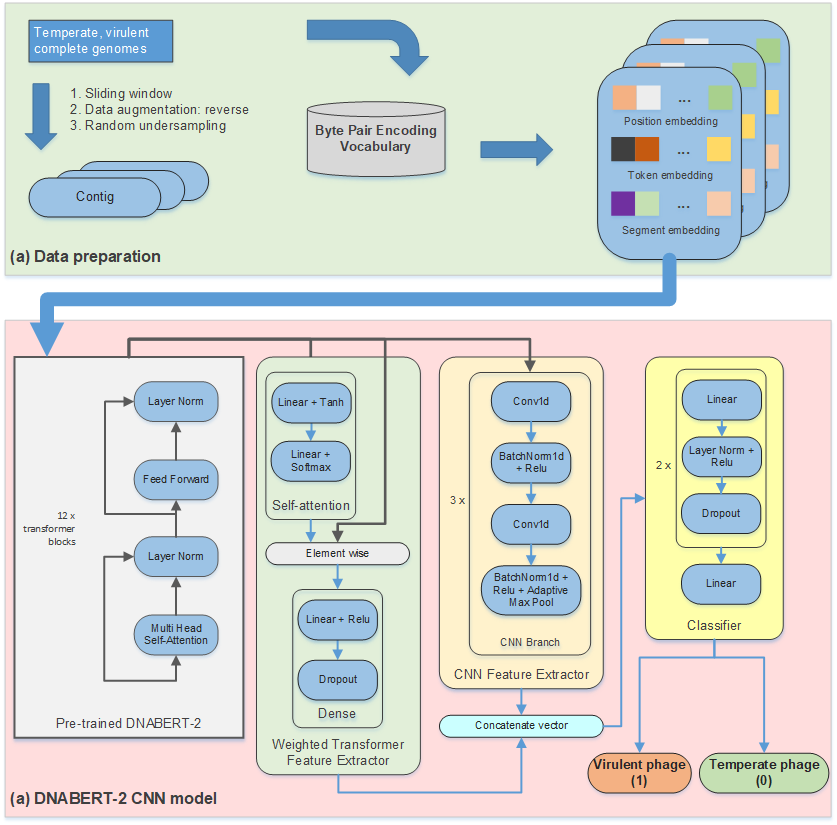
\includegraphics[width=\textwidth]{imgs/my_pipeline.png}
    \caption{Tổng quan kiến trúc PhaBERT-CNN cho dự đoán lối sống thực khuẩn thể}
    \label{fig:phabert_cnn_overview}
\end{figure}

\subsection{Quy trình xử lý}

Quy trình xử lý một contig DNA qua PhaBERT-CNN bao gồm các bước sau:

\begin{enumerate}
    \item \textbf{Tokenization}: Chuỗi DNA được tokenize bằng BPE tokenizer của DNABERT-2, tạo ra chuỗi tokens có độ dài giảm ~5 lần so với chuỗi gốc

    \item \textbf{DNABERT-2 encoding}: Chuỗi tokens được đưa qua 12 transformer encoder layers, tạo ra contextualized embeddings 768-dimensional cho mỗi token

    \item \textbf{Multi-scale CNN feature extraction}: Embeddings được xử lý song song qua ba nhánh CNN với kernel sizes khác nhau, mỗi nhánh tạo ra 128-dimensional feature vector

    \item \textbf{Attention-based global pooling}: Embeddings cũng được xử lý qua attention mechanism để tạo ra 128-dimensional global feature vector

    \item \textbf{Feature fusion}: Bốn feature vectors (3 từ CNN + 1 từ attention) được concatenate thành 512-dimensional composite representation

    \item \textbf{Classification}: Composite features được đưa qua classification head để tạo ra binary logits, sau đó áp dụng sigmoid để có xác suất dự đoán
\end{enumerate}

\subsection{Ưu điểm của kiến trúc}

Kiến trúc PhaBERT-CNN có những ưu điểm sau:

\begin{itemize}
    \item \textbf{Complementary feature extraction}: CNN nắm bắt local patterns, attention nắm bắt global context, kết hợp tạo ra representations phong phú

    \item \textbf{Multi-scale awareness}: Các kernel sizes khác nhau cho phép mô hình nhận diện patterns ở nhiều mức độ trừu tượng

    \item \textbf{Adaptive attention}: Mô hình tự động học vùng nào trong chuỗi quan trọng cho phân loại, không cần annotation thủ công

    \item \textbf{End-to-end learning}: Toàn bộ pipeline được tối ưu hóa cùng lúc, đảm bảo các thành phần hoạt động hài hòa

    \item \textbf{Transfer learning}: Tận dụng kiến thức từ DNABERT-2 pre-training, giảm nhu cầu về labeled data
\end{itemize}

Các sections tiếp theo sẽ trình bày chi tiết về từng thành phần của phương pháp PhaBERT-CNN.
